\documentclass[xcolor=x11names,compress]{beamer}

%% General document %%%%%%%%%%%%%%%%%%%%%%%%%%%%%%%%%%
\usepackage{ucs}     % unicode 
\usepackage[utf8x]{inputenc}  % utf-8
\usepackage[ngerman, english]{babel}  % new german spelling 
\usepackage[T1]{tipa}
\usepackage{ragged2e}
\usepackage{graphicx}
\usepackage{tikz}
\usetikzlibrary{decorations.fractals}
\usepackage{enumitem}
\usepackage{gb4e}
\usepackage{qtree}
\usepackage{soul}
\usepackage{bbding}
\usepackage{booktabs}
\usepackage{color}
\usepackage{fixltx2e}
%%%%%%%%%%%%%%%%%%%%%%%%%%%%%%%%%%%%%%%%%%%%%%%%%%%%%%


%% Beamer Layout %%%%%%%%%%%%%%%%%%%%%%%%%%%%%%%%%%
\useoutertheme[subsection=false,shadow]{miniframes}
\useinnertheme{default}
\usefonttheme{serif}
\usepackage{palatino}

\setbeamerfont{title like}{shape=\scshape}
\setbeamerfont{frametitle}{shape=\scshape}

\setbeamercolor*{lower separation line head}{bg=DeepSkyBlue4} 
\setbeamercolor*{normal text}{fg=black,bg=white} 
\setbeamercolor*{alerted text}{fg=red} 
\setbeamercolor*{example text}{fg=black} 
\setbeamercolor*{structure}{fg=black} 
 
\setbeamercolor*{palette tertiary}{fg=black,bg=black!10} 
\setbeamercolor*{palette quaternary}{fg=black,bg=black!10} 

\renewcommand{\(}{\begin{columns}}
\renewcommand{\)}{\end{columns}}
\newcommand{\<}[1]{\begin{column}{#1}}
\renewcommand{\>}{\end{column}}
%%%%%%%%%%%%%%%%%%%%%%%%%%%%%%%%%%%%%%%%%%%%%%%%%%


\begin{document}

%\documentclass{beamer}
%\usepackage{beamerthemesplit} 
%\usetheme{Goettingen}
%\usecolortheme{seahorse}
%\section{\scshape{\scshape Gliederung}
\begin{frame}
\title{\textbf{Semantic Role Labeling}}
%subtitle{}
\date{
	\begin{tikzpicture}[decoration=Koch curve type 2] 
		\draw[DeepSkyBlue4] decorate{ decorate{ decorate{ (0,0) -- (2,0) }}}; 
	\end{tikzpicture}  
	\\
	\vspace{0cm}
	\today
}

% \author{Arne Binder, Robert B\"arhold,\\
% 	{\it Humboldt Universität zu Berlin}\\
% 	Enrique Manjavacas\\
% 	{\it Freie Universität Berlin}\\
% }


\author[shortname]{Arne Binder \inst{1} \and Robert Bärhold \inst{1} \and Enrique Manjavacas \inst{2}}
\institute[shortinst]{\inst{1} Humboldt Universität zu Berlin\and %
                      \inst{2} Freie Universität Berlin}


\titlepage
\end{frame}
\begin{frame}
	\frametitle{Gliederung}
	\tableofcontents
	%[pausesections]
\end{frame}


\section{\scshape Theoretischer Hintergrund und Motivation}
	\frame{
		\frametitle{Argumentstruktur}
		%Beispielverb - zweiseitige Argumentstruktur
		% wie wir schon wissen, bestimmen Verben die zusaetzlichen Satzelementen zunachst hinsichtlich der Anzahl und Form. 
		% das resultierende Verhaltniss lautet Praedikat-Argument.
		\begin{itemize}[itemsep=3ex]
		\item<1->  \glqq{}ich kam\grqq{} \only<2->{[\textsubscript{PP+Dat} \textit{nach Rom}]}\\
						\vspace{0.7mm}
				   \glqq{}ich sah\grqq{} \only<3->{[\textsubscript{NP+Acc} \textit{die Armee}]}\\
				   		\vspace{0.7mm}
				   \glqq{}ich siegte\grqq{} \only<4->{[\textsubscript{PP+Acc} \textit{\"uber Pompeius}]}\\

		\item<5-> $\Longrightarrow$ Verben (als Pr\"adikate) bestimmen die Anzahl und Form ihrer Komplementen (Argumenten).
		\end{itemize}
	}

	
	\frame{
		\frametitle{thematische Rollen}
		% from the verb (lexical items) to the situation expressed thereby
		\begin{itemize}[itemsep=2ex]
			\item<1-> $\Longrightarrow$ Darüber hinaus bestimmen Verben die \glqq{}Art der Beteiligung\grqq{} der Mitspieler.
			\begin{itemize}[itemsep=1.5ex]%[label=$-$]
				\item<1-> \glqq{}ich\only<2-4>{\textsubscript{\textit{AGENS}}} kam nach Rom{\grqq{}}
				\item<3->  \glqq{}ich\only<4->{\textsubscript{\textit{EXPERIENCIER}}} sah die Armee{\grqq{}}
			\end{itemize}
		\end{itemize}
	}

	\frame{
		\frametitle{Frames und Frame elements}
		% from the situations to the verbs that evoke them
		% more exhaustive description of situation, great possibility to generalize over linguistic data
		% thematische Rollen sind Generalisierungen/abstraktionen \"uber die Bedeutung eines Satzgliedes in einer konkreten Verbverbindung.
		% 
			\begin{itemize}[label=$\bullet$,itemsep=1.5ex]
				\item Fokus wird nicht auf die Argumentstruktur gelegt sondern auf die Situation (Frame), die durch Sprache hervorgerufen wird.
				\item Auch andere Wortarten au\ss er Verben sind pr\"adikatwertig. 
				\begin{itemize}[label=$-$,itemsep=1ex]
					\item Bei Nominalisierung (Caesars Sieg \"uber Pompeius) 
					\item auch nicht nominalisierte Nomina (Frau, Mann ...)
				\end{itemize}
			\end{itemize}
	}
	
	\frame{
		\frametitle{Motivation}
			\begin{itemize}[label=$\bullet$,itemsep=1.5ex]
				\item Rollen sind die letzten Bausteinen, auf die die semantische Information eines Satzes basiert.
				\item Informationextraktion 
			\end{itemize}
		%Anwendungsbeispiele 
		%Informationextraktion,...
		%Warum Rollen? theoretisches Beispiel
		%nicht aufschreiben, aber sagen - the linguists scarcity problem, zu viele daten zu wenige linguisten
	}

\section{\scshape Problemstellung}

	\frame{
		\frametitle{Problemstellung}
		\centering
		$\Longrightarrow$Automatische Bestimmung von Rollen
		%%\vspace{1cm} 
		%\fbox{\parbox{\dimexpr \linewidth - 2\fboxrule - 2\fboxsep}{
		%\fbox{\parbox{\linewidth}{		
		\alert{Lassen sich semantische Rollen anhand von lexikalischen und syntaktischen Informationen eines Satzes automatisch bestimmen?}
		% }}
		%box rum blauer Rahmen
	}

	\frame{
		\frametitle{Corpus: Salsa 2.0}
		\begin{itemize}[label=$\bullet$,itemsep=1.5ex]
			\item<1->
			Erstellt von der Universität Saarland %Referenz
			% weiterentwicklung des SALSA 1.0
			\item<2->
			Basiert auf dem TIGER-Korpus %Referenz
			\begin{itemize}[label=$-$,itemsep=1ex]
				\item Treebank über Zeitungsartikel
				\item NEGRA Tag-Set
				\item
					viele syntaktische Informationen:\\ 
					Pos-Tag, morphologische \& lemma-Informationen
			\end{itemize}
			\item<3->
			Enthält: ~24.000 Sätze mit 648 Prädikaten %target-word
			\item<4->
			Prädikate: Nomen \& Verben

		\end{itemize}
	%	annotierung genau beschreiben (saetzengrenzen etc...)
	}	
	
	\frame{
		\frametitle{Corpus: Salsa 2.0}
		%Beispielbild von Salto: kurzer Satz mit edge-labels
	}


\section{\scshape Umsetzung}
	\frame{
		\frametitle{Einschränkungen}
		\begin{figure}
		\centering
		%@enrique: bitte einfügen!
		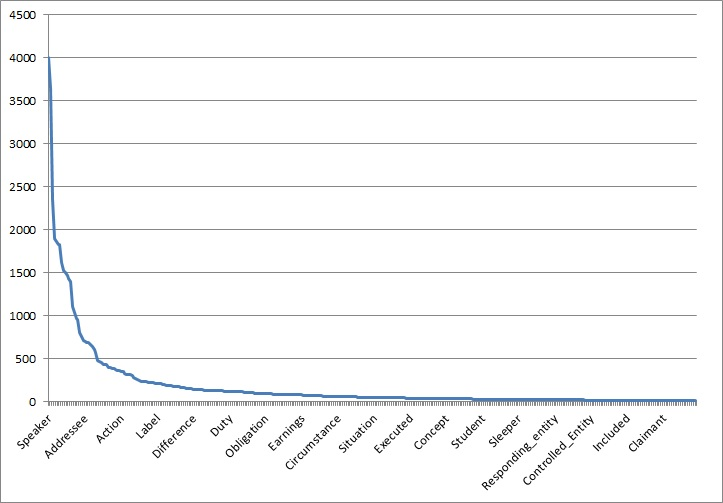
\includegraphics[scale=0.37]{images/roleFrequency.jpg}
		\caption{Verteilung der Rollen}
		\end{figure}
		%schöner Pfeil
		$\Longrightarrow$Betrachtung der Top-10 Rollen		
	}

	\frame{
		\frametitle{Herangehensweise}
		\begin{itemize}[label=$\bullet$,itemsep=1.5ex]
			\item Ansatz von Jurafsky und Gildea
			\begin{itemize}[label=$-$,itemsep=1ex]
				\item Analyse des Korpus auf Struktur, Aufbau, Häufigkeitsverteilungen
				\item Classifier: Naïve Bayes Classifier
				\item Angelehnte Features
			\end{itemize}
		\end{itemize}
	}

	\frame{
		\frametitle{Einschränkungen (Forts.)}
		\begin{itemize}[label=$\bullet$,itemsep=1.5ex]
			\item<1-> Top-10 Rollen

			%\vspace{1cm}
			\item<2-> Keine Frames
			\begin{itemize}[label=$-$,itemsep=1ex]
				\item Disambiguierung zu komplex
			\end{itemize}

			%\vspace{1cm}
			\item<3->Target-Lemma muss bekannt sein
			\begin{itemize}[label=$-$,itemsep=1ex]
				\item Keine Abstraktion für ungesehene Targets
			\end{itemize}
		\end{itemize}
	}
	

	\frame{
		\frametitle{Prinzipieller Ablauf}
		\begin{itemize}
			\item<1->
			\begin{figure}
				%@enrique: bitte einfügen!
				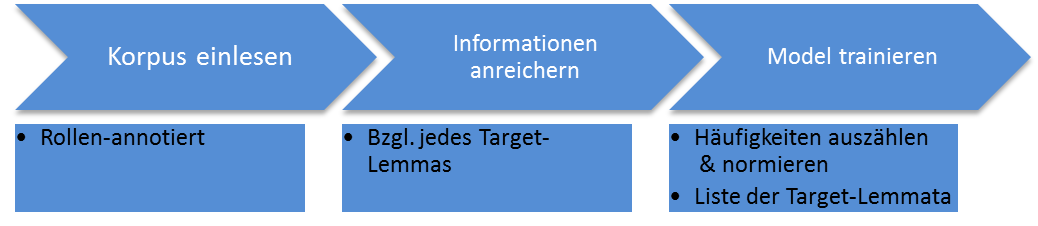
\includegraphics[scale=0.5]{images/ablaufLernen.png}
				\caption{Training}
			\end{figure}
			\item<2->
			\begin{figure}
				%@enrique: bitte einfügen!
				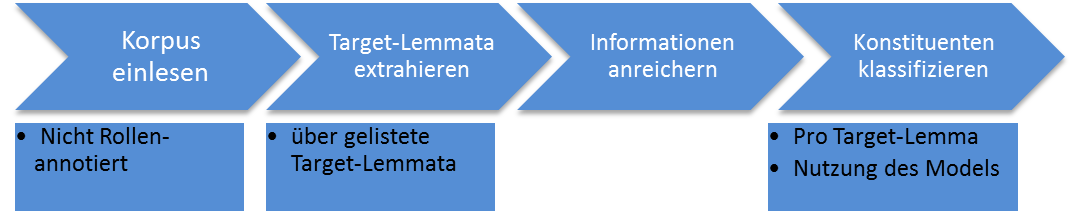
\includegraphics[scale=0.5]{images/ablaufAnnotate.png}
				\caption{Klassifikation}
			\end{figure}
		\end{itemize}
		%Keine Rolle
		%smoothing: 0.000001; threshold for frame: P(R1..Rk) > e^(-600)
	}

	\frame{
 % Kommentar in der E-Mail an Leser: Features einzeln mit einem Bild kurz erklären statt KOmpakt + Beispiel danach
		\frametitle{Features}
		\begin{itemize}[label=$\bullet$,itemsep=1.5ex]
			\item<1-> Synt. Kategorie
			\begin{itemize}[label=$-$,itemsep=1ex]
				\item Nonterminal: phrasale Kategorie
				\item Terminal: POS-Tag
			\end{itemize}
			
			%\vspace{1cm}
			\item<2-> Pfad: über synt. Kategorien
			\begin{itemize}[label=$-$,itemsep=1ex]
				\item Zusammenfassen von Replikaten 
				\item Ignorieren von Konjunktionen
			\end{itemize}

			%\vspace{1cm}
			\item<3-> Position
			\begin{itemize}[label=$-$,itemsep=1ex]
				\item Position relativ zum Target
			\end{itemize}
		\end{itemize}
	}

	\frame{
		\frametitle{Features (2)}
		\begin{itemize}[label=$\bullet$,itemsep=1.5ex]
			\item<1-> Kopf-Lemma
			\begin{itemize}[label=$-$,itemsep=1ex]
				\item Syntaktisches Zentrum einer Phrase %TODO
				\item wird regelbasiert gesucht
				%terminal =  eigenes lemma als head
			\end{itemize}

			%\vspace{1cm}			
			\item<2-> Nachbar-Kopf-Lemma
			\begin{itemize}[label=$-$,itemsep=1ex]
				\item Kopf der einbettenden Konstituente
			\end{itemize}

			%\vspace{1cm}
			\item<3-> Kombination: Synt. Kat. \& Pfad
		\end{itemize}
	}

	\frame{
		\frametitle{Features (3)}
		%Features an Beispielsatz von Salsa-Corpus (Salto-Satz) erklären
	}

	\frame{ % ZEILENABSTAND
		\frametitle{Probleme}
		\begin{itemize}[label=$\bullet$,itemsep=1.5ex]
			\item Deutsch: relativ freie Verschiebung von Konstituenten %Subjekt nicht auf die Vorfeldposition beschränkt....
			\item Kopf nicht überall definiert (NEGRA Tag-Set)
			\item Querverbindung im Syntaxgraph % KOAN BAUM
			\begin{itemize}[label=$-$,itemsep=1ex]
				\item Ich ging nach Haus' und aß Abendbrot. (Bild?)
			\end{itemize}			
			\item Target im Satz identifizieren
			\begin{itemize}[label=$-$,itemsep=1ex]
				\item Den Vortrag \textit{auf die lange Bank schieben.}
				\item Ich \textit{brach} den Ast \textit{ab.}
			\end{itemize}			
		\end{itemize}
	}	


\section{\scshape Evaluation}
	\frame{
		\frametitle{Evaluation}
		\begin{itemize}[label=$\bullet$,itemsep=1.5ex]
			\item Target-Lemma muss vorhanden sein
			\begin{itemize}[label=$-$,itemsep=1ex]
				\item keines gefunden: Satz komplett ignoriert
			\end{itemize}
%da wir eine feste liste von target lemmata nutzen und nicht auf ungesehene targets abstrahieren koennen beruecksichtigen wird bei der evaluation nur 
%frame elements mit dem bezug auf ein (im Model) bekanntes target. counts erklaeren und ausgeben 
			\item Nutzung des F-Mesaure
			\begin{itemize}[label=$-$,itemsep=1ex]
				\item Sehr, sehr häufig: keine Rolle % accuracy dadurch unpassend
			\end{itemize}

			\item Precision
			\begin{itemize}[label=$-$,itemsep=1ex]
				\item P = \#(Korrekte Rolle klassifiziert) / \\ \#Klassifiziert mit Rolle)
			\end{itemize}				

			\item Recalll
			\begin{itemize}[label=$-$,itemsep=1ex]
				\item R = \#(Korrekte Rolle klassifiziert) / \\ \#(Konstituenten mit Rolle)
			\end{itemize}				
		\end{itemize}
	}

	\frame{
		\frametitle{Auswertung bezüglich dreier Kenngrößen}
		\begin{itemize}[label=$\bullet$,itemsep=1.5ex] %TODO: should be enumerate
			\item Konstituente wurde korrekte Rolle zugewiesen
			\begin{itemize}[label=$-$,itemsep=1ex]
				\item Exakte Übereinstimmung
			\end{itemize}

			\item Konstituente wurde eine bel. Rolle zugewiesen
			\begin{itemize}[label=$-$,itemsep=1ex]
				\item Unabhängig von der Rolle
			\end{itemize}

			\item Korrekte Rolle wurde im Satz gefunden
			\begin{itemize}[label=$-$,itemsep=1ex]
				\item Unabhängig der Position im Satz
			\end{itemize}
		\end{itemize}
		% das letzte geht mehr auf die Rollenzählung ein, die ersten beiden sind für Konstituenten
	}

	\frame{
		\begin{figure}
			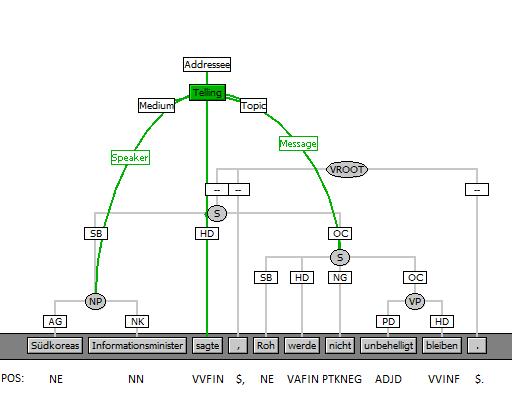
\includegraphics[scale=0.5]{images/s6544.png}
			\caption{annotiertes Beispielsatz}
		\end{figure}%TODO Beispielsatz von Salto wieder nutzen, muss mind. 2 Rollen haben
	}


	\frame{
		\frametitle{Ergebnisse}
		\begin{itemize}[label=$\bullet$,itemsep=1.5ex]
		  \item Korpus: Top-10 Rollen
		  \begin{itemize}[label=$-$,itemsep=1ex]
			  \item $\sim$ 14000 Sätzen
			  \item $\sim$ 22500 Konstituenten mit einer Rolle
		  \end{itemize}
		\end{itemize}

		%\vspace{1cm}
		\begin{table}
			\small
			\caption{Ergebnisse einer 5-fach Kreuzvalidierung}
			\begin{tabular}{r|c|c|c}
			  	\toprule
			  	Typ						& \textbf{Precision} & \textbf{Recall} & \textbf{F-Measure} \\
			  	\midrule
				Exaktes Match 			&  0,51 $\pm$ 0,02 & 0,81 $\pm$ 0,02 & 0,62 $\pm$ 0,02 \\
				Unabhängig (Rolle)		&  0,67 $\pm$ 0,03 & 0,85 $\pm$ 0,02 & 0,75 $\pm$ 0,02 \\
				Unabhängig (Position)	&  0,55 $\pm$ 0,02 & 0,88 $\pm$ 0,02 & 0,68 $\pm$ 0,02 \\
				\bottomrule
			\end{tabular}
		\end{table}

		\begin{center}
			\small
			Angabe: Ergebniswert (gerundet) $\pm$ Standardabweichung
		\end{center}
	}

	\frame{
		\frametitle{Einordnung der Ergebnisse}
		\begin{itemize}[label=$\bullet$,itemsep=1.5ex]
			\item Erstes SRL-Projekt auf dem SALSA 2.0 Korpus
			%\vspace{1cm}
			\item Universität Saarland: Projekt auf dem SALSA 1.0 Korpus
			\begin{itemize}[label=$-$,itemsep=1ex]
				\item Prec.: 0.761  $\vert$ Recall: 0.496  $\vert$ F-Mesaure: 0.600
				\item Vorgehen \& Evaluation unklar
			\end{itemize}

			%\vspace{1cm}
			\item Target-Lemma muss vorhanden sein
			\begin{itemize}[label=$-$,itemsep=1ex]
				\item 92\% der Konstituenten im Korpus ignoriert 
				%TODO  = (IDrefs overall - classified idrefs) / idrefs overall * 100
			\end{itemize}	
			\begin{itemize}
				\item $\Longrightarrow$ besserer Recall $\Longrightarrow$ besserer F-Measure
			\end{itemize}
		\end{itemize}
	}

	\frame{
		\centering
		\begin{Large} 
			Vielen Dank für die Aufmerksamkeit! \\
			%\vspace{1cm}
		\end{Large}
		\vspace{1cm}
		\begin{tikzpicture}[decoration=Koch curve type 2] 
			\draw[DeepSkyBlue4] decorate{ decorate{ decorate{ (0,0) -- (2,0) }}}; 
		\end{tikzpicture} \\
			Fragen?
	}

	\frame{
		\frametitle{Referenzen}
		...% TODO
	}

	\frame{
		%empty frame

	}

	\frame{
		\frametitle{Backup}

	}	


	% \frame{
	% 	\frametitle{Auswertung bezüglich dreier Kenngrößen}
	% 	\begin{enumerate}
	% 		\item Konstituente wurde korrekte Rolle zugewiesen
	% 		\begin{itemize}
	% 			\item Exakte Übereinstimmung
	% 		\end{itemize}	

	% 		\item Konstituente wurde eine bel. Rolle zugewiesen
	% 		\begin{itemize}
	% 			\item Unabhängig von der Rolle
	% 		\end{itemize}	
			
	% 		\item Korrekte Rolle wurde im Satz gefunden
	% 		\begin{itemize}
	% 			\item Unabhängig der Position im Satz
	% 		\end{itemize}	
	% 	\end{enumerate}
	% 	% das letzte geht mehr auf die Rollenzählung ein, die ersten beiden sind für Konstituenten
	% }

	% \frame{
	% 	% Beispielsatz von Salto wieder nutzen, muss mind. 2 Rollen haben
	% }


	% \frame{
	% 	\frametitle{Durchführung}
	% 	\begin{itemize}
	% 		\item 5-fache Kreuzvalidierung % je ein paar weg

	% 		% Gesamtergebnis + Standardabweichung

	% 	\end{itemize}
	% }

	% \frame{
	% 	\frametitle{Einordnung der Ergebnisse}
	% 	\begin{itemize}
	% 		\item Erstes SRL-Projekt auf dem SALSA 2.0 Korpus
	% 		\item Universität Saarland: Projekt auf dem SALSA 1.0 Korpus
	% 		\begin{itemize}
	% 			\item Prec.: 0.761 | Recall: 0.496 | F-Mesaure: 0.600
	% 			\item Vorgehen \& Evaluation unklar
	% 		\end{itemize}

	% 		%\vspace{1cm}
	% 		\item Target-Lemma muss vorhanden sein
	% 		\begin{itemize}
	% 			\item xx \% an Konstituenten im Goldstandard wurden ignoriert %TODO
	% 			\item --> führt zu besserem Recall -> F-Measure
	% 		\end{itemize}	
	% 	\end{itemize}
	% }

	% \frame{
	% 	Vielen Dank für die Aufmerksamkeit!
	% }

	% \frame{
	% 	\frametitle{Referenzen}
	% 	...%todo
	% }

	% \frame{
	% 	%empty frame

	% }

	% \frame{
	% 	\frametitle{Backup}

	% }	

%%%%%%%%%%%%%%%%%%%%%%%%%%%%%%%%%%%%%%%%%%%%




% \frame{
% \frametitle{What are semantic  roles?}
% \begin{itemize}
% 	\item<2->
% 			\begin{xlist}
% 			\ex
% 			\gll Peter gibt Karl Geld.\\
% 			\footnotesize
% 			\textcolor{blue}{\textit{SOURCE}}
% 			\footnotesize
% 			{}
% 			\footnotesize
% 			\textcolor{blue}{\textit{RECIPIENT} }
% 			\footnotesize
% 			\textcolor{blue}{\textit{THEMA}}
% 			\\
% 			%\vspace{1cm}
% 	\item<3->
			
% 			\gll Karl bekommt Geld von Peter.\\
% 			\footnotesize
% 			\textcolor{blue}{\textit{RECIPIENT}}
% 			\footnotesize
% 			{}
% 			\footnotesize
% 			\textcolor{blue}{\textit{THEMA}}
% 			\footnotesize
% 			\textcolor{blue}{\textit{SOURCE}}
% 			\\
% 			\end{xlist}

			
% \end{itemize}
% }



% \section{\scshape[Why Semantic Roles?]{}
% \frame{
% \frametitle{Why Semantic Roles?}
% \begin{itemize}
% 	\item<1-> \begin{block}{\textbf{Information Extraction}}
% 	\begin{itemize}
% 		\item "Paul hat seine Mutter get\"otet."
% 	\end{itemize}
% 	\end{block}
% 	%\vspace{1cm}
% 	\item<2-> \begin{block}{\textbf{Metaphernanalyse}}
% 	\begin{itemize}
% 		\item "Paul hat seine Mutter unter die Erde gebracht."
% 	\end{itemize}
% 	\end{block}
% \end{itemize}
% }

% \section{\scshape[Our goal]{}
% \frame{
% \frametitle{Our goal}
% \begin{itemize}
% 	\item<1-> Automatic Semantic Role Labeling
% 	\item<2-> Language: German
% 	\item<3-> Corpus: SALSA 2.0 (based on TIGER Corpus \& FrameNet)
% 	\item<4-> Framework: LingPipe 
% 	%\vspace{1cm}
% 	\item<5-> \textbf{References:} C.J. Fillmore (Frame Semantics), D. Jurafsky \& D. Gildea (first implementation of a Semantic Role Labeler)
	
% \end{itemize}
% }



 \end{document}
